\documentclass[border=0.2cm]{standalone}
 
% More defined colors
\usepackage[dvipsnames]{xcolor}
 
% Required package
\usepackage{tikz}
\usetikzlibrary{positioning}
 
 
\begin{document}
 
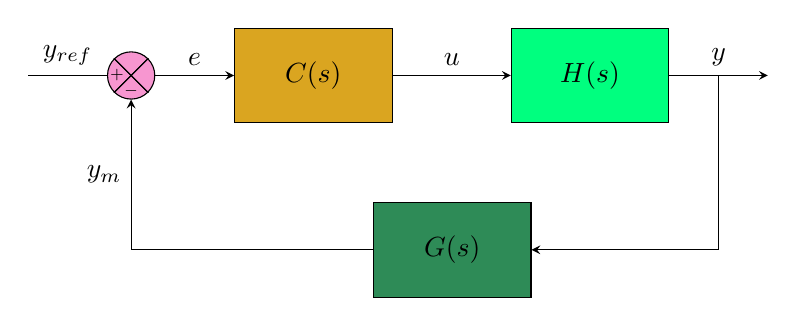
\begin{tikzpicture}
 
\node[draw,
    circle,
    minimum size=0.6cm,
    fill=Rhodamine!50
] (sum) at (0,0){};
 
\draw (sum.north east) -- (sum.south west)
    (sum.north west) -- (sum.south east);
 
\draw (sum.north east) -- (sum.south west)
(sum.north west) -- (sum.south east);
 
\node[left=-1pt] at (sum.center){\tiny $+$};
\node[below] at (sum.center){\tiny $-$};
 
\node [draw,
    fill=Goldenrod,
    minimum width=2cm,
    minimum height=1.2cm,
    right=1cm of sum
]  (controller) {$C(s)$};
 
\node [draw,
    fill=SpringGreen, 
    minimum width=2cm, 
    minimum height=1.2cm,
    right=1.5cm of controller
] (system) {$H(s)$};
 
\node [draw,
    fill=SeaGreen, 
    minimum width=2cm, 
    minimum height=1.2cm, 
    below right= 1cm and -0.25cm of controller
]  (sensor) {$G(s)$};
 
% Arrows with text label
\draw[-stealth] (sum.east) -- (controller.west)
    node[midway,above]{$e$};
 
\draw[-stealth] (controller.east) -- (system.west) 
    node[midway,above]{$u$};
 
\draw[-stealth] (system.east) -- ++ (1.25,0) 
    node[midway](output){}node[midway,above]{$y$};
 
\draw[-stealth] (output.center) |- (sensor.east);
 
\draw[-stealth] (sensor.west) -| (sum.south) 
    node[near end,left]{$y_m$};
 
\draw (sum.west) -- ++(-1,0) 
    node[midway,above]{$y_{ref}$};
 
 
\end{tikzpicture}
 
\end{document}